% Two-column conference preamble: an 8-page body cap, references after.
%
% The body is single-spaced two-column 10pt. References are pushed onto a fresh
% page by \clearpage so the body page count is unambiguous and machine-checkable
% -- paper/build.py reads the page number of the references label and reports
% it, and the test suite fails if it exceeds the cap.
%
% Generated from the corresponding .md by paper/build.py. Do not edit.

\documentclass[10pt,twocolumn,letterpaper]{article}

\usepackage[margin=0.75in,columnsep=0.28in]{geometry}
\usepackage{amsmath}
\usepackage{amssymb}
\usepackage{booktabs}
\usepackage{graphicx}
\usepackage{array}
\usepackage{calc}
\usepackage{caption}
\usepackage{microtype}
\usepackage{balance}
\usepackage[hidelinks]{hyperref}
\usepackage{newunicodechar}

\graphicspath{{../results/figures/}}

\captionsetup{font=small,labelfont=bf,skip=4pt}
\setlength{\tabcolsep}{4pt}
\renewcommand{\arraystretch}{1.08}
\setlength{\emergencystretch}{3em}
\setlength{\parskip}{0pt}
\setcounter{secnumdepth}{0}
\urlstyle{same}

% Tighter section spacing than the article default; two columns at 10pt leave
% no room for the default 3.5ex gaps.
\usepackage{titlesec}
\titlespacing*{\section}{0pt}{1.6ex plus .2ex}{0.7ex}
\titlespacing*{\subsection}{0pt}{1.2ex plus .2ex}{0.5ex}
\titleformat*{\section}{\large\bfseries}
\titleformat*{\subsection}{\normalsize\bfseries}

% pandoc emits these
\providecommand{\tightlist}{%
  \setlength{\itemsep}{0pt}\setlength{\parskip}{0pt}}
\providecommand{\pandocbounded}[1]{#1}
\newcounter{none}

\newunicodechar{Ω}{\ensuremath{\Omega}}
\newunicodechar{α}{\ensuremath{\alpha}}
\newunicodechar{×}{\ensuremath{\times}}
\newunicodechar{−}{\ensuremath{-}}
\newunicodechar{≥}{\ensuremath{\ge}}
\newunicodechar{≈}{\ensuremath{\approx}}
\newunicodechar{→}{\ensuremath{\rightarrow}}
\newunicodechar{↔}{\ensuremath{\leftrightarrow}}
\newunicodechar{₀}{\ensuremath{_0}}
\newunicodechar{₂}{\ensuremath{_2}}
\newunicodechar{₅}{\ensuremath{_5}}
\newunicodechar{⁻}{\ensuremath{^-}}
\newunicodechar{⁵}{\ensuremath{^5}}
\newunicodechar{⁷}{\ensuremath{^7}}
\newunicodechar{é}{\'e}

\title{\vspace{-3ex}Annotation independence and reference coverage in the evaluation of drug--drug interaction screens: 17,375 drug pairs in 22 years of FAERS\vspace{-1ex}}
\author{[TODO: author list and affiliations]}
\date{}

\begin{document}
\twocolumn[\begin{@twocolumnfalse}
\maketitle
\begin{abstract}
\noindent Computational screens over spontaneous reporting databases routinely claim to enrich for genuine drug--drug interactions (DDIs), and routinely evaluate that claim against reference lists the investigators wrote themselves. We show that this practice produces apparent enrichment whether or not the method works, and we report a negative discovery result from a screen whose sensitivity is independently characterised. Screening 17,375 drug pairs for myotoxicity across the complete public history of the FDA Adverse Event Reporting System (20,274,416 cases, 41,889 events), a pipeline that recovers 12 of 16 label-verified positive controls returned \textbf{1,022 signals against 1,212 expected by chance} once the chance rate is allowed to vary with marginal strength instead of being held at its pooled value --- that is, \textbf{fewer signals than chance predicts}. A uniform rate gives 874 and suggests a modest excess; the false-positive rate in fact varies by an order of magnitude across the screen. Pooled enrichment of known interaction pairs appears significant (2.02×, 95\% CI 1.59--2.55), but every positive-control drug also appears on the list defining ``known pair''; \textbf{restricting to pairs containing no control drug leaves enrichment at 1.12× (0.69--1.81)}. The result holds under an independent, endpoint-specific reference built from FDA labelling (1.23×, falling to 1.045 after stratification on co-report count), under restriction to label-covered pairs (1.067, 0.292--1.972), under stratification on reported hospitalisation, and under adjustment for marginal strength. The band designated in advance as where a novel interaction would appear shows enrichment \textbf{below} unity (0.749, 0.567--0.973). A temporal-stability filter that appeared to be a powerful discriminator admits 0.093\% of negative controls, implying 16.1 era-stable pairs by chance against 19 observed. Separately, we find the evaluation references themselves are the binding constraint: \textbf{11 of the 200 screened ingredients (5.5\%) have no FDA label at all}, making \textbf{9.8\% of pairs} undocumentable by construction, and the screen's highest-ranked pair by event rate --- atorvastatin + fusidic acid, 155 events in 185 co-reports --- is a contraindicated interaction that no available reference contained. Claims that this class of screen discovers novel interactions should be treated with scepticism until the annotation used to evaluate them is demonstrably independent of the control set used to build them.
\end{abstract}
\vspace{2ex}
\end{@twocolumnfalse}]


\section{1. Introduction}\label{introduction}

Disproportionality screens over spontaneous reports are the standard instrument for post-marketing drug--drug interaction surveillance. A screen of this kind is typically evaluated by asking whether its signals are enriched for pairs already known to interact, and the reference list defining ``known'' is frequently assembled by the same investigators who assembled the positive controls used to validate the method.

That arrangement has a structural problem. If the control drugs also populate the reference list, then any method that recovers its controls will show enrichment against the reference, regardless of whether it generalises to pairs nobody nominated in advance. The enrichment measures the overlap between two author-written lists, not the method's discovery capability.

This paper reports what happens when that circularity is removed. We screen 17,375 drug pairs for myotoxicity across the complete public FAERS history, using a pipeline whose sensitivity and false-positive rate are independently characterised, and evaluate the resulting signals against three annotations of increasing independence --- the authors' own curated list, FDA labelling for any endpoint, and FDA labelling restricted to this endpoint --- each applied both to all pairs and to pairs containing no positive-control drug, plus a further restriction to pairs whose two labels both exist.

The result is negative, and it is reported as the finding. We also report why the negative result is bounded by the \emph{references} rather than by the method --- an observation with direct consequences for how such screens should be evaluated.

\textbf{Contributions.} (i) A demonstration that author-written annotation produces apparent enrichment independent of method performance, with the effect quantified (2.02× → 1.12×). (ii) A negative discovery result robust across three annotations, two scopes and four confounder adjustments. (iii) Quantification of structural reference blindness --- 5.5\% of screened ingredients, 9.8\% of pairs --- including the agent in the screen's highest-ranked pair. (iv) A worked case in which the screen's top-ranked pair is a genuine contraindicated interaction invisible to every available reference.

\section{2. Background}\label{background}

\textbf{Reference sets.} TWOSIDES (Tatonetti et al., 2012) is derived from FAERS itself and is unsuitable as an independent reference for a FAERS screen. DrugBank is licensed and was unavailable to us. The ONC high-priority DDI list (Phansalkar et al., 2012) \emph{is} openly available --- a 15-row table --- and we retrieved and examined it. It is not usable here, for a reason specific to its construction: it is expressed as \emph{drug-class} pairs (``HMG Co-A reductase inhibitors ↔ CYP3A4 inhibitors''), so applying it requires an ingredient-to-class mapping that would itself be author-written, reintroducing the circularity at issue. Only one of the 15 entries concerns myotoxicity, and the source explicitly excluded the gemfibrozil--statin interaction on the grounds that clinical benefit outweighs risk.

A curated, ingredient-level, severity-graded DDI compendium remains unavailable, and that absence is the single largest limitation of this evaluation.

\textbf{Disproportionality and the estimand.} The measures used here follow the shrinkage logic of Bate et al.~(1998) and DuMouchel (1999). The screen is run on an additive (excess-risk) null rather than the multiplicative null underlying Ω (Norén et al., 2008). At the conventional threshold Ω₀₂₅ \textgreater{} 0 the additive null recovers 12 of 16 positive controls against 4 for Ω. \textbf{That comparison is made at very different error rates, not matched ones}: among pairs as strongly associated as the positive controls, Ω fires on 2.2\% of non-interacting pairs and the additive null on 9.3\%, against a nominal 2.5\% for both. Equalising the rates reduces the recovery gap from eight pairs to one or two. The companion paper establishes this; what matters here is that \textbf{the screen's operating point is empirical rather than nominal} --- the threshold used below (+0.436) was calibrated against negative controls and validated out of sample, not taken from the measure's conventional cut.

\textbf{That validation is specification-dependent, and this paper's foundation inherits the dependence.} Two binary design choices exist --- the event tier (\texttt{core}, specific; \texttt{broad}, inclusive) and the drug role policy (\texttt{primary}, suspect roles only; \texttt{sensitivity}, wider). All four arms were computed, and the additive null's advantage is not uniform across them (Table 1). It holds under either widening alone and vanishes under both together. \texttt{core}/\texttt{primary} is pre-specified in configuration and is the arm underlying every result below.

\begin{table}[t]
\centering
\small
\caption{Positive-control recovery across all four design specifications. The screen evaluated in this paper runs under the pre-specified arm.}
\begin{tabular}{@{}llrr@{}}
\toprule
Tier & Role policy & Additive & Multiplicative \\
\midrule

\textbf{core} & \textbf{primary} \emph{(pre-specified)} & \textbf{12/16} & \textbf{4/16} \\
core & sensitivity & 12/16 & 4/16 \\
broad & primary & 11/16 & 4/16 \\
\textbf{broad} & \textbf{sensitivity} & \textbf{6/16} & \textbf{6/16} \\
\end{tabular}
\end{table}

This matters for what follows. A negative discovery result draws its force from the demonstration that the same pipeline finds known interactions; if that demonstration is specification-dependent, so is the null result reported here. We state the dependence rather than inherit the headline figure without it.

\section{3. Methods}\label{methods}

\section{3.1 Pipeline and population}\label{pipeline-and-population}

All 90 quarterly FAERS archives (2004Q1--2026Q2, 328,476,258 rows) were parsed under an audited schema map, validated by referential integrity (\textbf{0 orphan rows}), and reduced to 20,293,421 distinct cases by six-stage deduplication. After excluding 19,005 cases listing more than 20 drugs --- a cap adopted because such cases contribute 34.7\% of all drug pairs at a 4× enriched event rate --- the analysis population is \textbf{20,274,416 cases carrying 41,889 myotoxicity events (0.207\%)}. Drug entries were resolved to active ingredients (98.0\% of 73,960,283 rows) and the event defined by 23 hand-curated MedDRA Preferred Terms in 10 concepts.

\section{3.2 The screen and its bands}\label{the-screen-and-its-bands}

The screen covers the top 200 ingredients by co-reporting with the event, giving 17,375 pairs with at least three co-reports.

\textbf{Not every entry in that vocabulary can form a drug pair.} The selection rule is applied mechanically to FDA's resolved active-ingredient field, and four of the 200 entries are placeholders that field supplies where it cannot resolve a moiety --- \texttt{UNSPECIFIED\ INGREDIENT}, \texttt{HERBALS}, \texttt{INSULIN\ NOS} and \texttt{CANNABIS\ SATIVA\ SUBSP\ INDICA\ TOP}. A further three pairs are one moiety with itself, valproate reaching the vocabulary as \texttt{VALPROATE}, \texttt{VALPROIC\ ACID} and \texttt{DIVALPROEX}. Together these account for \textbf{719 pairs (4.1\% of the screen), of which 38 signal and 122 fall in the \texttt{plausible} band}.

We do not remove them from the primary analysis: the drug-selection rule was fixed in advance, and excluding terms after seeing results would be a researcher degree of freedom. The sensitivity is reported instead (§4.4), and it is small. Each pair is assigned in advance to one of four bands: \texttt{positive\_control} (one of the 16 validated controls), \texttt{known\_pair} (both drugs on the author-curated implicated list), \texttt{plausible} (one implicated drug plus an unimplicated partner --- designated in advance as where a novel interaction would appear), and \texttt{unsupported} (neither implicated).

The signal threshold was calibrated against the full pool of 16,138 generated negative controls and validated out of sample by 500 half-splits: held-out threshold +0.429 and held-out false-positive rate \textbf{5.03\% (95\% CI 4.37--5.74\%)} against the in-sample +0.436.

The threshold depends on the gamma-posterior shrinkage constant, α = 0.5, which is conventional but \textbf{could not be verified against the primary source} (paywalled and unread by the authors). The companion paper varies it over a 20-fold range with the threshold recalibrated at each value: control recovery varies by two pairs and the signal count by 7\%. No conclusion here turns on it, but the dependency is real and is stated rather than assumed away.

\section{3.3 The independent reference}\label{the-independent-reference}

Because the investigators wrote both the positive control set and the ``known pair'' list, a second annotation was built that they did not author. For each screened ingredient we retrieved the most recent FDA product label via openFDA and recorded which other screened ingredients are named in its DRUG INTERACTIONS, CONTRAINDICATIONS or WARNINGS AND PRECAUTIONS sections. Labels are cached, fixing the reference against future revisions.

This is independent of the authors but \textbf{not} of FAERS: labelling is informed by post-marketing surveillance, so it cannot establish that a signal was found independently of the data. It establishes only that the annotation was not written by us, which is the circularity at issue.

Labels also warn by class (``strong CYP3A4 inhibitors'') as often as by name, so the reference is under-sensitive and biases measured enrichment downward. That is the conservative direction for a claim that enrichment \emph{exists}, and the \textbf{anti}-conservative direction for this paper's claim, which is that it does not: attenuating a ratio toward unity moves it toward our own conclusion. Section 4.3 therefore reports the analysis restricted to pairs whose two labels both exist.

\section{3.4 Statistics}\label{statistics}

\textbf{A limitation of the negative-control pool.} The generator excludes any pair in which both drugs appear on the myotoxicity-implicated list --- a guard against seeding the null set with true positives, but one that removes exactly the configuration every positive control has. The resulting pool sits at a median log₂(RR\_A × RR\_B) of 0.56 against 8.23 for the positive controls, and only 0.1\% of it reaches their interquartile floor. Any rate estimated from it and applied uniformly across the screen will misstate the bands, which is why §4.1 reports the strength-matched alternative. The companion paper constructs a purpose-built high-marginal pool and measures the error rates directly.

Binomial tests are \textbf{not} used for inference: with 200 drugs, each drug sits in 199 pairs, so pair outcomes are strongly dependent. Significance is assessed by a permutation test holding the pair graph and observed signal pattern fixed while randomising which drugs are annotated as implicated (10,000 permutations). Interval estimates for enrichment use a cluster bootstrap resampling \textbf{drugs} rather than pairs; the pairwise interval is anticonservative and is labelled as such wherever reported.

\section{4. Results}\label{results}

\section{4.1 The screen returns little above chance}\label{the-screen-returns-little-above-chance}

Of 17,375 pairs, \textbf{1,022} exceeded threshold. A pooled chance expectation --- the held-out false-positive rate of 5.03\% applied uniformly --- gives 874 (95\% CI 759--997), suggesting a modest excess.

\textbf{That calculation assumes the false-positive rate is constant across the screen, and it is not.} Measured on the negative controls it runs from 0.93\% to 10.91\% across quintiles of marginal strength, and the four bands differ systematically on that variable (median log₂(RR\_A × RR\_B) of 2.85, 4.16, 5.32 and 8.15). Matching each screened pair to the observed rate among negative controls of similar marginal strength:

\begin{table}[t]
\centering
\small
\caption{Observed signals against a pooled and a strength-matched chance expectation.}
\begin{tabular}{@{}lrrrr@{}}
\toprule
band & tested & observed & pooled (5.03\%) & strength-matched \\
\midrule

unsupported & 11,887 & 717 & 598 & \textbf{824} \\
plausible & 4,930 & 228 & 248 & \textbf{348} \\
known pair & 543 & 66 & 27 & \textbf{39} \\
positive control & 15 & 11 & 1 & 1 \\
\textbf{total} & 17,375 & \textbf{1,022} & \textbf{872} & \textbf{1,212} \\
\end{tabular}
\end{table}

\textbf{Under the strength-matched expectation the screen returns fewer signals than chance predicts} --- 1,022 against 1,212 --- and only \texttt{known\_pair} exceeds its own expectation. The apparent excess under the pooled figure is an artefact of averaging a rate that varies by an order of magnitude.

This does not change the paper's conclusion; it sharpens it. But the strength-matched column extrapolates into the high-marginal bands from a thin and unrepresentative slice of the negative pool (§3.4), so the 1,212 figure carries real uncertainty. That the uniform assumption is wrong does not.

\(\Omega_{\mathrm{add},025}\) is a shrinkage bound, not a \emph{p}-value, and carries no false-discovery guarantee; the calibrated threshold stands in for one. As an independent check, a one-sided Poisson test of each triple count against its additive expectation with Benjamini--Hochberg control at \emph{q} = 0.05 yields \textbf{1,147 discoveries}, and every one of the 1,022 shrinkage signals is among them. The shrinkage rule is the more conservative of the two, so no conclusion below depends on the absence of a formal correction.

\begin{table}[t]
\centering
\small
\caption{Signal rate by pre-specified band.}
\begin{tabular}{@{}llrl@{}}
\toprule
Band & Signalled & Rate & Enrichment (95\% CI) \\
\midrule

Positive control & 11/15 & 73.3\% & 12.16 (8.89--16.63) \\
Known pair & 66/543 & 12.2\% & 2.02 (1.59--2.55) \\
\textbf{Plausible} & 228/4,930 & 4.6\% & \textbf{0.77 (0.66--0.89)} \\
Unsupported & 717/11,887 & 6.0\% & 1.00 (0.90--1.11) \\
\end{tabular}
\end{table}

\section{4.2 The apparent enrichment is the circularity}\label{the-apparent-enrichment-is-the-circularity}

A drug-level permutation test gives pooled enrichment 2.29× (\emph{p} = 0.0012) under the author-curated annotation, so the pooled effect is not an artefact of pair dependence alone. \textbf{Under the independent FDA-labelling annotation the same test is not significant} (2.80×, \emph{p} = 0.14). Dependence-aware significance is present for the annotation the investigators wrote and absent for the one they did not.

All 12 positive-control drugs are among the 64 drugs defining ``known pair'', and that list was written by the same investigators. Restricting to pairs containing \textbf{no} positive-control drug reduces enrichment from 2.02× to \textbf{1.12× (95\% CI 0.69--1.81)} against an unsupported reference of 1.00 --- indistinguishable from unity. \textbf{The pooled 2.02× is essentially entirely attributable to pairs containing a drug the investigators had already nominated.}

Two corrections were required before the independent reference could be used. First, a label documents that two drugs interact, not that the interaction causes \emph{this} event: 82\% of name-matched pairs are documented for an unrelated endpoint, and omeprazole + warfarin --- a real CYP2C19 interaction affecting INR --- was being counted as a hit in a myotoxicity screen. The endpoint-specific reference additionally requires a myotoxicity term within 600 characters of the partner drug's name, giving 709 pairs that still capture 16/16 positive controls. Second, documented pairs are co-reported about three times more often than undocumented ones (median 202 versus 69, Mann--Whitney \emph{p} = 2 × 10⁻⁷⁵), and co-report count drives power directly, so results are also stratified on co-report decile.

\begin{table}[t]
\centering
\small
\caption{Enrichment under every annotation scheme.}
\begin{tabular}{@{}
  >{\raggedright\arraybackslash}p{(\linewidth - 8\tabcolsep) * \real{0.2000}}
  >{\raggedright\arraybackslash}p{(\linewidth - 8\tabcolsep) * \real{0.2000}}
  >{\raggedright\arraybackslash}p{(\linewidth - 8\tabcolsep) * \real{0.2000}}
  >{\raggedright\arraybackslash}p{(\linewidth - 8\tabcolsep) * \real{0.2000}}
  >{\raggedright\arraybackslash}p{(\linewidth - 8\tabcolsep) * \real{0.2000}}@{}}
\toprule
\begin{minipage}[b]{\linewidth}\raggedright
Annotation
\end{minipage} & \begin{minipage}[b]{\linewidth}\raggedright
Scope
\end{minipage} & \begin{minipage}[b]{\linewidth}\raggedright
Signalled
\end{minipage} & \begin{minipage}[b]{\linewidth}\raggedright
Enrichment (95\% CI)
\end{minipage} & \begin{minipage}[b]{\linewidth}\raggedright
Strat.
\end{minipage} \\
\midrule

Author-curated & Pooled & 66/543 & 2.02 (1.59--2.55) & --- \\
Author-curated & No control drug & 16/237 & \textbf{1.12 (0.69--1.81)} & --- \\
FDA, any endpoint & Pooled & 110/1,339 & 1.44 (1.19--1.75) & 1.24 \\
FDA, any endpoint & No control drug & 57/1,069 & 0.92 (0.71--1.20) & 0.75 \\
\textbf{FDA, myotoxicity} & Pooled & 48/240 & 3.52 (2.71--4.56) & 3.08 \\
\textbf{FDA, myotoxicity} & \textbf{No control drug} & 10/142 & \textbf{1.23 (0.67--2.24)} & \textbf{1.045} \\
\end{tabular}
\end{table}

All annotations agree. Pooled enrichment is real and, under the endpoint-specific reference, substantial (3.52×). \textbf{It vanishes once pairs containing a positive-control drug are removed.} The negative result does not depend on who wrote the reference, on whether the reference is endpoint-specific, or on the power confound.

\begin{figure}[htbp]
\centering
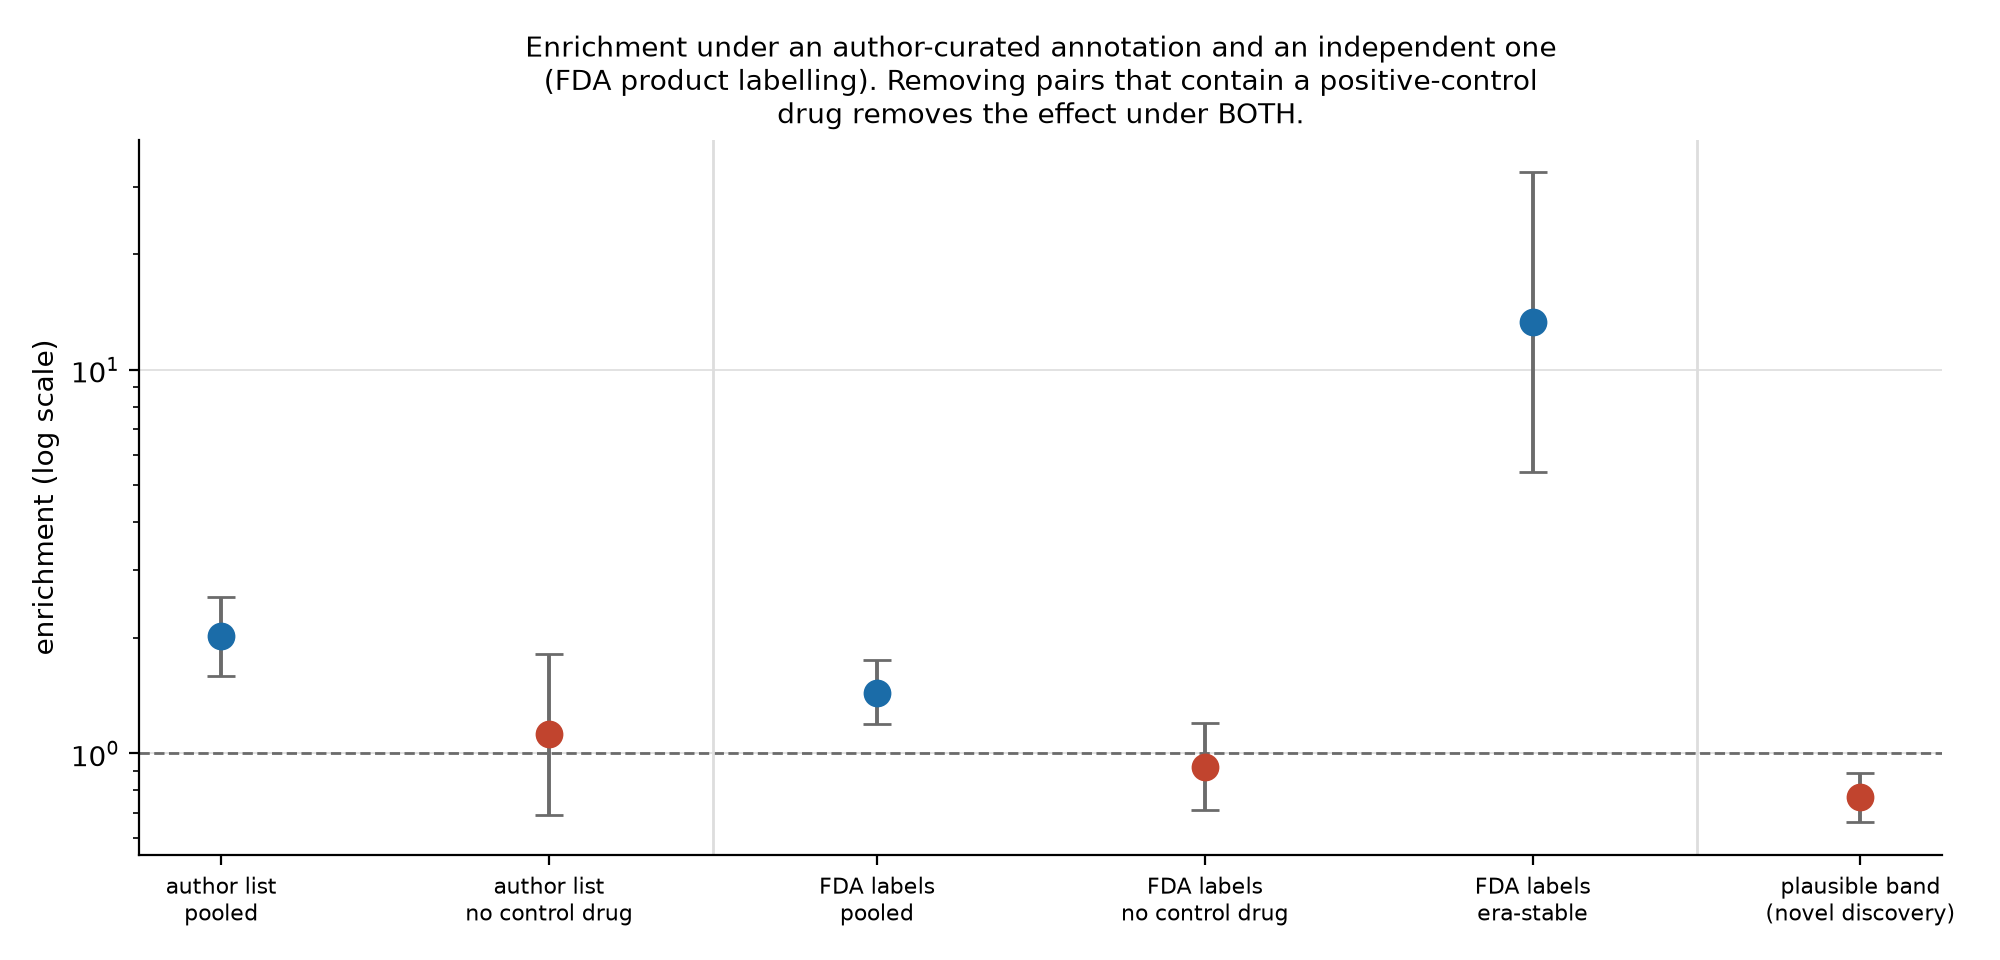
\includegraphics[width=0.85\linewidth]{figure3_band_enrichment.png}
\caption{\textbf{Band enrichment under two annotations.} Signal enrichment relative to unsupported pairs, log scale, with 95\% intervals. Points left of each divider are pooled; points right of it exclude pairs containing a positive-control drug.}
\label{fig:1}
\end{figure}

\section{4.3 The reference is structurally blind to part of the screen}\label{the-reference-is-structurally-blind-to-part-of-the-screen}

\textbf{11 of the 200 screened ingredients (5.5\%) have no FDA label in openFDA at all}, so no pair containing one can ever be documented. Because those 11 are well co-reported, they account for a disproportionate share of the pair space: \textbf{1,712 of 17,375 pairs (9.8\%)} are undocumentable by construction and fall into the denominator.

The gap is not random. It falls on agents without a current US marketing authorisation, and the one that matters for this endpoint is \textbf{fusidic acid}, whose statin combination is contraindicated in practice and is the screen's highest-ranked pair by event rate (§4.6).

Widening the reference beyond the screened set makes the coverage problem more visible without changing the screen: of the 800 ingredients for which labels were retrieved for the screen-size sensitivity analysis (§4.3), 138 (17.2\%) have none, and those include \textbf{cerivastatin} --- a statin withdrawn worldwide for rhabdomyolysis with gemfibrozil --- together with \textbf{bezafibrate, ciprofibrate} and \textbf{telithromycin}. None of the four entered the top-200 screen, so they do not bear on the result reported here; they indicate that any wider screen would inherit a larger version of the same blindness.

Restricting to non-control pairs where \emph{both} labels exist, so that ``undocumented'' means the label is silent rather than absent, gives enrichment \textbf{1.24 (0.68--2.26)} crude and \textbf{1.067 (0.292--1.972)} stratified. \textbf{The negative result is unchanged by the correction}, but the reference's coverage is a property of US marketing status rather than of pharmacology and should be read that way.

\textbf{Power.} The comparison rests on 142 documented non-control pairs, with 83\% power at a true enrichment of 2.5× but only 57\% at 2.0× and 23\% at 1.5×. The correct reading is therefore ``no enrichment above roughly 2.24×'' --- the upper confidence bound --- rather than ``no enrichment''. Extending the label reference to 800 drugs raises this to 444 documented pairs; the crude interval then excludes unity, but the drug-level cluster bootstrap does not at any screen size (1.045, 1.311, 1.265 at top-200, -400 and -800). The dependence-respecting interval is the one to read, and \textbf{the negative result survives the power increase}, excluding enrichment above roughly 1.988×.

\begin{figure}[htbp]
\centering
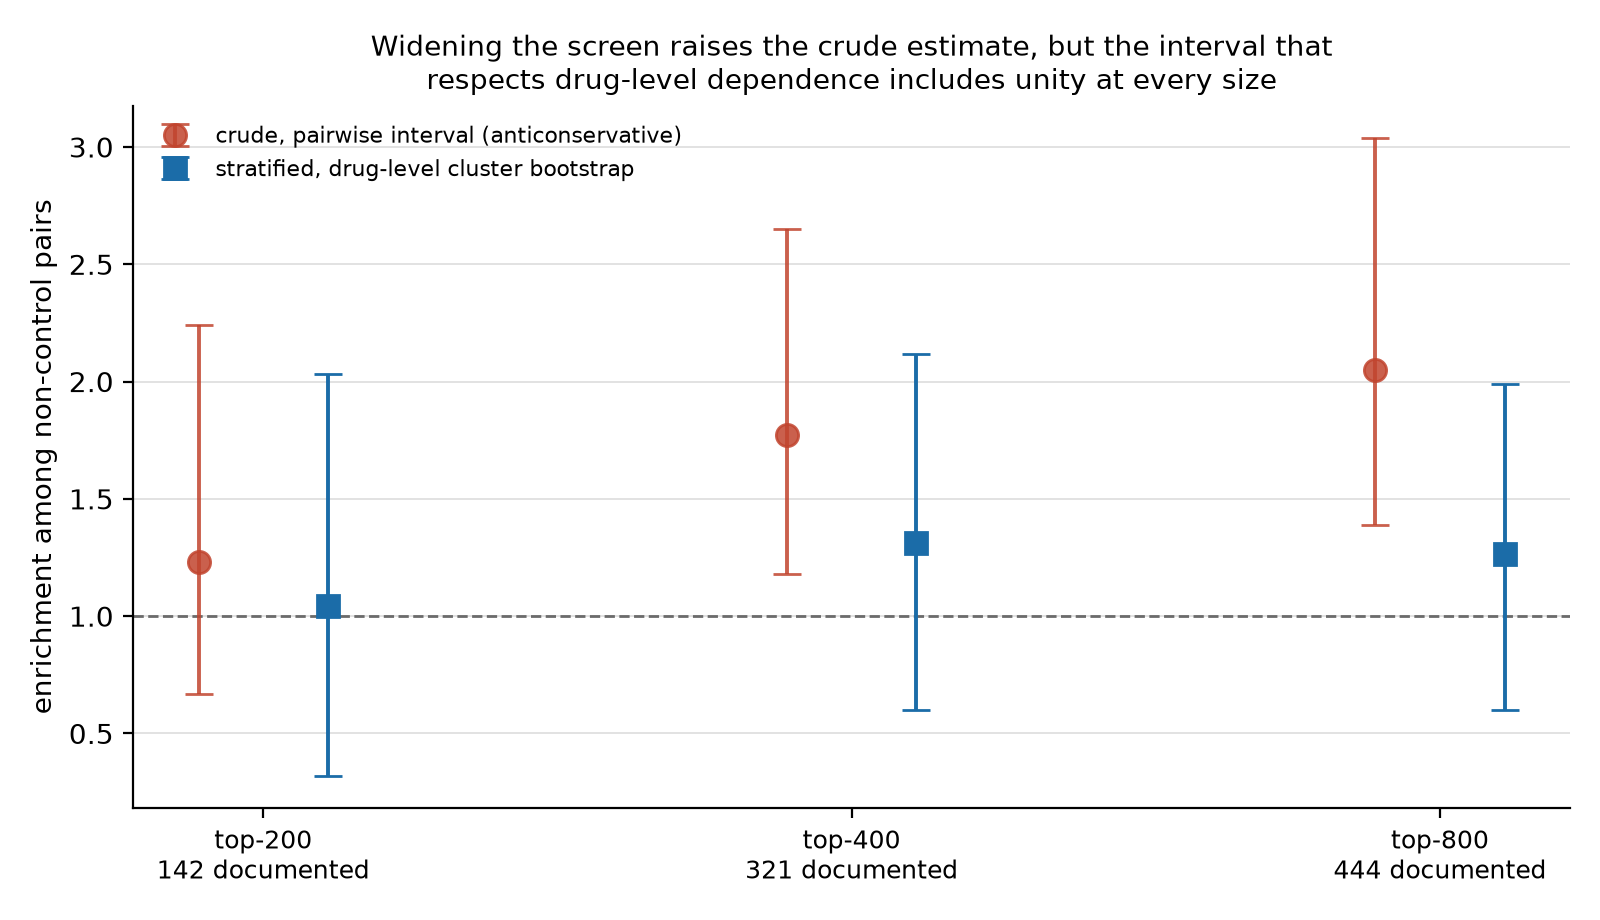
\includegraphics[width=0.85\linewidth]{figure7_screen_size_power.png}
\caption{\textbf{Screen size and power.} Enrichment among non-control pairs at three screen sizes, under the pairwise interval (red, anticonservative) and the drug-level cluster bootstrap (blue).}
\label{fig:2}
\end{figure}

\section{4.4 The discovery band is below unity, and stays there}\label{the-discovery-band-is-below-unity-and-stays-there}

The \texttt{plausible} band --- one implicated drug plus an unimplicated partner, designated in advance as where a novel interaction would appear --- has enrichment \textbf{0.77 (0.66--0.89)}, significantly \emph{below} unity.

Because the bands differ systematically in the marginal strength of their constituent drugs (median \(\log_2(RR_A \times RR_B)\) of 2.85 unsupported, 4.16 plausible, 5.32 known pair, 8.15 positive control), and marginal strength drives the expected count, this comparison requires adjustment for that covariate as well as for co-report count. Applying the same Mantel--Haenszel machinery to deciles of marginal strength: \texttt{plausible} moves from 0.767 to \textbf{0.749 (0.567--0.973)}, still below unity, while \texttt{known\_pair} moves from 2.015 to 1.835 (0.99--2.989) and its interval now touches unity. The confound is small and non-monotone (quintile signal rates 3.7\%, 7.2\%, 6.6\%, 5.2\%, 6.7\%). \textbf{The discovery band's deficit survives adjustment}; the known-pair band's apparent 2× does not survive intact, consistent with the circularity argument above.

\textbf{Vocabulary hygiene.} The 719 pairs that cannot be interactions (§3.2) barely move the result: \texttt{plausible} enrichment goes from \textbf{0.766 to 0.752} and \texttt{known\_pair} from \textbf{2.015 to 1.995} when they are removed. The band conclusions do not depend on them. They do, however, matter for reading individual pairs --- 122 sit in the \texttt{plausible} band, and a pair naming \texttt{UNSPECIFIED\ INGREDIENT} is uninterpretable however it scores.

\textbf{Confounding by inpatient status.} Two adjustments were attempted and only the second is adequate. Excluding cases containing any of 30 hand-picked procedural or critical-care agents removes 275,205 cases --- \textbf{1.4\% of the population} --- and leaves band enrichment essentially unchanged (0.76 → 0.75). That is not evidence that inpatient confounding is absent: perturbing 1.4\% of the data cannot exclude a confounder, and a null was near-guaranteed before the analysis ran. FAERS records the outcome directly, and stratification on \texttt{outc\_cod\ =\ \textquotesingle{}HO\textquotesingle{}} (5,709,555 reports) splits the population into two large, comparable halves.

\begin{table}[t]
\centering
\small
\caption{Screen stratified on reported hospitalisation.}
\begin{tabular}{@{}lrrrr@{}}
\toprule
Stratum & Cases & Event rate & Plausible & Known pair \\
\midrule

Hospitalised & 4,274,465 & 0.669\% & \textbf{0.639} & 1.839 \\
Not hospitalised & 15,999,951 & 0.083\% & \textbf{0.825} & 1.885 \\
\end{tabular}
\end{table}

The 8-fold difference in event rate confirms hospitalisation is a genuine confounder, unlike the 1.4\% proxy which could not have detected one. \textbf{Both strata reproduce the result.}

\section{4.5 Temporal stability does not survive validation}\label{temporal-stability-does-not-survive-validation}

Requiring the signal in all three eras reduces 1,022 pairs to \textbf{19}. Each era bin is scored against the same threshold calibrated on the full 22 years, and a bin holds roughly a third of the cases, so the filter is far stricter than ``the signal is present in each era'' --- it selects on co-report count as much as on temporal consistency.

Of the 19, nine carry prior support. But the same filter applied to the 6,471 negative controls that also enter the screen admits \textbf{6 of them (0.093\%, 95\% CI 0.039--0.191\%)}, implying \textbf{16.1 era-stable pairs by chance (95\% CI 6.8--33.2) against 19 observed}. \textbf{The count is not distinguishable from chance.} An earlier version of this analysis reported the filter as a principal contribution, on the basis of an enrichment figure computed without ever applying it to negative controls.

\begin{figure}[htbp]
\centering
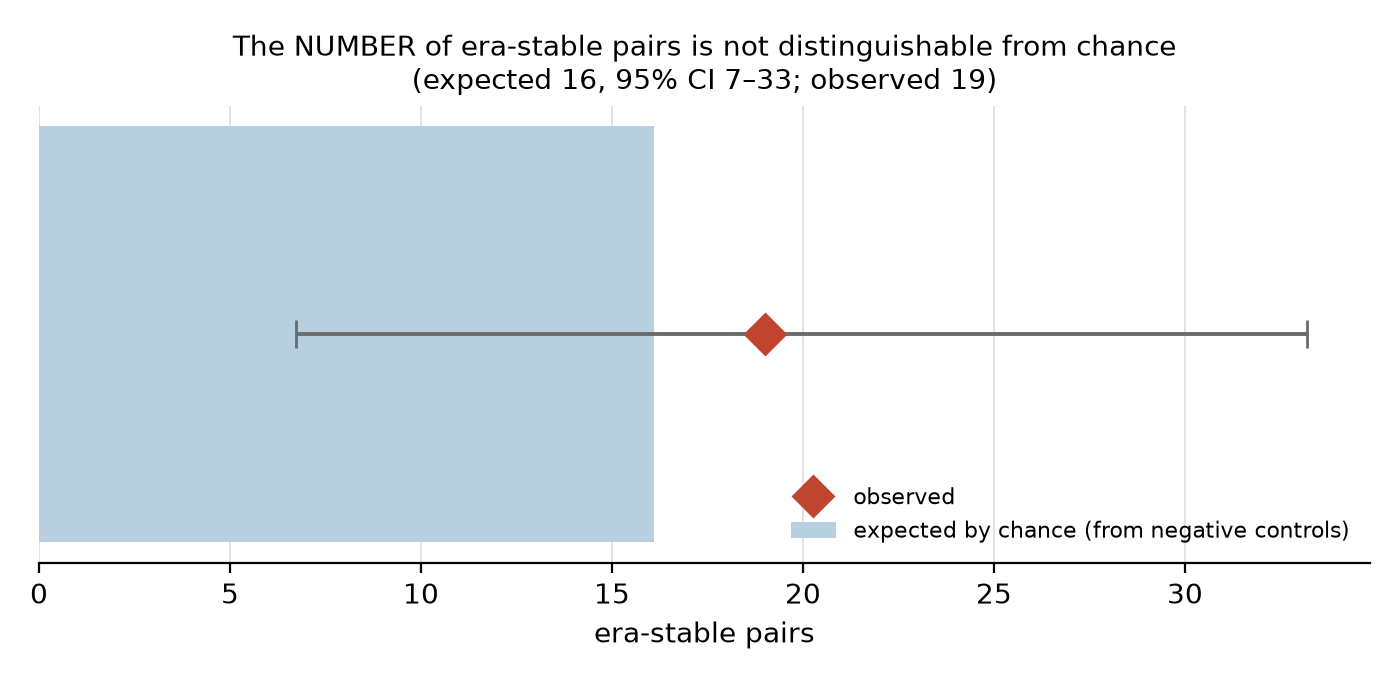
\includegraphics[width=0.85\linewidth]{figure4_era_stability.png}
\caption{\textbf{Era-stability against chance.} Era-stable pairs observed (red diamond) against the number expected by chance (bar, 95\% interval) from applying the same filter to negative controls.}
\label{fig:3}
\end{figure}

A composition-based claim appeared to survive --- among era-stable pairs, 10 of 1,339 label-documented pairs signal against 9 of 16,036 undocumented, enrichment 13.31× (5.42--32.69). It does not withstand the two corrections applied to every other enrichment here (Table 4). \textbf{Once the reference is endpoint-specific and control drugs are removed, not one era-stable pair is documented.} The claim rested on the same circularity, which an earlier draft asserted this analysis had escaped. It had not. The count of era-stable pairs is separately shown to be an artefact of bin choice, running from 84 at two bins to 3 at five.

\begin{table}[t]
\centering
\small
\caption{Era-stable composition by reference and scope.}
\begin{tabular}{@{}llll@{}}
\toprule
Reference & Scope & Doc. signalled & Crude \\
\midrule

Any endpoint & All pairs & 10/1,339 & 13.31 (5.42--32.69) \\
Any endpoint & No control drug & 2/1,069 & 4.45 (0.90--22.0) \\
Endpoint-specific & All pairs & 8/240 & 51.9 (21.1--127.9) \\
\textbf{Endpoint-specific} & \textbf{No control drug} & \textbf{0/142} & \textbf{---} \\
\end{tabular}
\end{table}

\section{4.6 The top-ranked pair is an interaction no reference contained}\label{the-top-ranked-pair-is-an-interaction-no-reference-contained}

The eight era-stable pairs without prior support are statin proxies: most carry a statin, fibrate or colchicine on \textbf{88--100\%} of their event cases against a 40.5\% background, with paroxetine + valsartan, levothyroxine + valsartan, aspirin + metoprolol and aspirin + ramipril at exactly 100\%. These are markers for ``cardiovascular patient taking a statin''.

That explanation does \textbf{not} dispose of the two era-stable pairs in the \texttt{plausible} band (Table 5).

\begin{table}[t]
\centering
\small
\caption{The two era-stable pairs in the discovery band.}
\begin{tabular}{@{}
  >{\raggedright\arraybackslash}p{(\linewidth - 8\tabcolsep) * \real{0.1579}}
  >{\raggedleft\arraybackslash}p{(\linewidth - 8\tabcolsep) * \real{0.2105}}
  >{\raggedleft\arraybackslash}p{(\linewidth - 8\tabcolsep) * \real{0.2105}}
  >{\raggedleft\arraybackslash}p{(\linewidth - 8\tabcolsep) * \real{0.2105}}
  >{\raggedleft\arraybackslash}p{(\linewidth - 8\tabcolsep) * \real{0.2105}}@{}}
\toprule
\begin{minipage}[b]{\linewidth}\raggedright
Pair
\end{minipage} & \begin{minipage}[b]{\linewidth}\raggedleft
\emph{n}
\end{minipage} & \begin{minipage}[b]{\linewidth}\raggedleft
Events
\end{minipage} & \begin{minipage}[b]{\linewidth}\raggedleft
Rate
\end{minipage} & \begin{minipage}[b]{\linewidth}\raggedleft
Third implicated drug
\end{minipage} \\
\midrule

\textbf{Atorvastatin + fusidic acid} & 185 & 155 & \textbf{83.8\%} & \textbf{8.4\%} vs 48.7\% bg \\
Ciprofloxacin + simvastatin & 377 & 152 & 40.3\% & 44.7\% vs 48.7\% bg \\
\end{tabular}
\end{table}

Atorvastatin + fusidic acid is the \textbf{highest-event-rate pair in the entire screen} --- above every one of the 16 positive controls, the best of which reaches 71.0\% --- is era-stable across all three eras, exceeds its additive expectation, and is \emph{under}-represented for third-drug polypharmacy rather than over-represented. It is also a real and serious interaction: systemic fusidic acid with a statin is contraindicated.

It sits in the discovery band because \textbf{neither reference contains it}. Fusidic acid has no US marketing authorisation, so openFDA returns no label and no fusidic acid pair can ever be documented; it is also absent from the investigators' own implicated-drug list. The screen ranked a genuine contraindicated interaction first and both evaluation references were blind to it.

No pair identified by this screen constitutes a \emph{novel} interaction --- atorvastatin + fusidic acid is documented, not novel. But the claim that every era-stable pair traces to confounding is too strong, and the negative discovery result measures the references at least as much as the method.

\section{5. Discussion}\label{discussion}

\textbf{An evaluation whose annotation is written by the same investigators as the control set will show enrichment whether or not the method works.} The gap between 2.02× and 1.12× here is entirely that circularity, and it is large enough to convert a null result into an apparently significant one. Screens reporting enrichment against author-curated reference lists should be read accordingly, and reviewers should ask directly whether the annotation and the control set share authorship. The test is cheap: recompute enrichment over pairs containing no control drug.

\textbf{Reference quality, not method sensitivity, is the binding constraint.} The negative result survives every adjustment we could apply, but the fusidic acid case shows what those adjustments cannot fix. A reference whose coverage tracks marketing authorisation rather than pharmacology will be blind to precisely the agents that are withdrawn, non-US, or off-label --- a set enriched for exactly the safety signals a surveillance system exists to find. Measured sensitivity against such a reference is a lower bound of unknown tightness.

\textbf{Sensitivity is bracketed, not estimated.} Against author-selected controls the pipeline recovers 86\%; against label-selected controls, 12\%. The gap is not power --- recovery \emph{falls} as co-reporting rises, and the most heavily co-reported label-documented pairs show event rates at or below the database baseline, carrying class rather than pair-specific warnings. Neither figure is the sensitivity; they bracket it. Narrowing the bracket needs a severity-graded reference distinguishing pair-specific interactions from class warnings.

\textbf{Practical recommendations.} Report enrichment with control-drug pairs excluded. Use an annotation you did not author, and state its coverage as a fraction of the screened space. Apply the discovery filter to negative controls before reporting it as a discriminator. Use dependence-respecting intervals, since pairwise intervals over a screen where each drug appears in hundreds of pairs are anticonservative and can exclude unity where a cluster bootstrap does not.

\section{6. Limitations}\label{limitations}

The independent reference is FDA labelling, not a curated DDI database, and is absent entirely for 5.5\% of screened ingredients, which nonetheless account for 9.8\% of pairs. The measured false-positive rate remains an upper bound.

The negative result is bounded, not absolute: at the widest screen it rests on 444 documented non-control pairs, with approximately 70\% power at a true enrichment of 2.0 and 30\% at 1.5, excluding enrichment above roughly 1.988×. A real but modest enrichment would still be missed.

The 16 positive controls are author-selected and comprise five victim drugs rather than sixteen independent trials, so the sensitivity that anchors this evaluation carries a wide interval (50--100\% on the powered subset).

Screened drugs are selected on the outcome, which is selection on the dependent variable. Reselecting by total report volume does not change the conclusion, but that check leaves only 38 documented non-control pairs of which one signals, with a crude interval of 0.14--6.49 --- too little power to be reassuring, and we do not present it as such. The negative controls are drawn from the same selected universe and share any induced bias.

The analyses in Sections 4.3--4.6 are post-hoc, each added in response to a specific objection raised during internal review, and several changed the paper's conclusions. No multiplicity correction has been applied across them and the intervals are nominal.

No external reporting system was used. VigiAccess, the free public window onto VigiBase, groups results by active ingredient and continental region and exposes no drug-pair facility, so it cannot validate an interaction result at all; pair-level access requires a research agreement. Conclusions may be FAERS-specific. Spontaneous reporting has no exposure denominator: nothing here estimates risk, only reporting disproportionality.

\section{7. Conclusion}\label{conclusion}

A screen over the complete public FAERS history, using a pipeline that recovers 12 of 16 label-verified interactions at a characterised false-positive rate, finds no evidence of enrichment for genuine drug--drug interactions once the evaluating annotation is made independent of the control set. The apparent 2.02× enrichment falls to 1.12× on that single change, and the result holds under an independent endpoint-specific reference, under restriction to label-covered pairs, under stratification on reported hospitalisation, and under adjustment for marginal strength. A temporal-stability filter that appeared to be a strong discriminator is indistinguishable from chance once applied to negative controls.

The evaluation references are the binding constraint rather than the method: 5.5\% of screened ingredients have no label at all --- 9.8\% of pairs --- and the screen's top-ranked pair by event rate is a contraindicated interaction none of them contained. Claims that this class of screen discovers novel interactions should be treated with scepticism until the annotation used to evaluate them is demonstrably independent of the control set used to build them.

\section{Computational environment and reproducibility}\label{computational-environment-and-reproducibility}

A single workstation, macOS on Apple silicon; Python 3.14.6, DuckDB 1.5.5, pandas 3.0.5, PyArrow 25.0.0, NumPy 2.5.1, SciPy 1.18.0, matplotlib. Exact pinned versions accompany the code. Downloading the 90 archives takes roughly 30 minutes on a domestic connection, parsing 328,476,258 rows to Parquet about 3 minutes at 4 processes, and the full analysis about 12 minutes. Peak memory is bounded by a 10 GB DuckDB limit; no GPU is used.

Every stochastic procedure is seeded and the seeds are in the shipped configuration: the drug-level cluster bootstrap (20,000 draws for control recovery, 1,000 for enrichment intervals), the drug-level permutation test (10,000 permutations), the induced-correlation simulation (10,000 draws) and the 500-split threshold calibration. The pipeline is deterministic: two full runs produce byte-identical output, and this is checked rather than asserted.

\section{Data and code availability}\label{data-and-code-availability}

All code, configuration and result tables are available at
\url{https://github.com/edanmn/faers-ddi-rhabdomyolysis}. Every figure quoted in the Abstract and Results is generated into \texttt{results/canonical\_numbers.json} by a single deterministic run and asserted against this text by \texttt{tests/test\_canonical\_numbers.py}; pipeline statistics quoted in Methods are persisted under \texttt{audit.provenance} in the same file and asserted alongside them. Figures drawn from cited work are attributed and not regenerated. The pipeline is deterministic: two full runs produce byte-identical output.

\textbf{This is research code and a research result. It is not clinical guidance.}

\section{Acknowledgements}\label{acknowledgements}

{[}TODO{]}

\clearpage
\label{sec:endofbody}
\section{References}\label{references}

\begin{enumerate}
\def\labelenumi{\arabic{enumi}.}
\tightlist
\item
  Bate A, Lindquist M, Edwards IR, Olsson S, Orre R, et al.~A Bayesian neural network method for adverse drug reaction signal generation. \emph{Eur J Clin Pharmacol.} 1998;54(4):315--321. doi:10.1007/s002280050466
\item
  Banda JM, Evans L, Vanguri RS, Tatonetti NP, Ryan PB, Shah NH. A curated and standardized adverse drug event resource to accelerate drug safety research. \emph{Sci Data.} 2016. PMID 27193236.
\item
  DuMouchel W. Bayesian data mining in large frequency tables, with an application to the FDA spontaneous reporting system. \emph{Am Stat.} 1999;53(3):177--190. doi:10.1080/00031305.1999.10474456
\item
  Fusaroli M, et al.~Enhancing transparency in defining studied drugs: the open-source living DiAna dictionary for standardizing drug names in the FAERS. \emph{Drug Saf.} 2024;47:271--284.
\item
  Norén GN, Sundberg R, Bate A, Edwards IR. A statistical methodology for drug--drug interaction surveillance. \emph{Stat Med.} 2008;27(16):3057--3070. PMID 18344185. doi:10.1002/sim.3247
\item
  Phansalkar S, et al.~High-priority drug--drug interactions for use in electronic health records. \emph{J Am Med Inform Assoc.} 2012;19(5):735--743. PMID 22539083. doi:10.1136/amiajnl-2011-000612
\item
  Tatonetti NP, Ye PP, Daneshjou R, Altman RB. Data-driven prediction of drug effects and interactions. \emph{Sci Transl Med.} 2012. PMID 22422992. doi:10.1126/scitranslmed.3003377
\item
  VanderWeele TJ, Knol MJ. A tutorial on interaction. \emph{Epidemiol Methods.} 2014;3(1):33--72. doi:10.1515/em-2013-0005
\end{enumerate}


\end{document}
